\section{Indledning}

Denne rapport er udarbejdet af 6 studerende, der læser til civilingeniør i robotteknologi på SDU, det tekniske fakultet.\\

Det vil være en fordel hvis læseren af denne rapport har en grundlæggende kendskab til programmering og elektronik. Dette skyldes at projektet hovedsageligt går ud på at benytte elektronik og programmering til at løse opgaven.\\

I dette projekt er formålet at finde en metode til at opnå den hurtigste omgangstid på en vilkårlig bane. Der vil tages højde for hastighed i sving og på langside. Bilen udstyres med forskellige sensorer for at kunne kortlægge banen og vide hvornår målstregen passeres. Til sidst er der foretaget en vurdering af projektet i helhed.\\

Projektet er lavet i en gruppe, hvor arbejdsopgaver fordeles. Hvert medlem har dog ansvar for at sætte sig ind i dele, de ikke selv har været en del af. Gruppen har haft møde en mindst gang ugentligt, hvor der blev fremlagt fremskridt, diskussion af problemer undervejs samt uddelegering af nye arbejdsopgaver. Gruppen har i forløbet haft flere møder med vejleder, for at diskutere retning og eventuelle spørgsmål er blevet afklaret.\\

Rapporten er opbygget kronologisk og de forskellige kapitler, der har relevans for hinanden, vil ligge samlet. Således er der en rødtråd igennem rapporten.\\


\subsection{Problemformulering}

Vi ønsker at ombygge en scalextric bil til at kunne kører autonomt på en ukendt bane. Den skal selv formå at opmåle banen og derudfra regulere sine egne parametre, med det formål at opnå den hurtigst mulige omgangstid.
\begin{itemize}
	\item Hvordan får vi bilen til at bremse?
	\item Hvordan får vi bilen til at hold en jævn hastighed?
	\item Hvordan får vi mappet banen op?
	\item Hvordan får bilen til at reagere på det givne map?
\end{itemize}

\subsection{Kravspecifikation}

Vi har fået stillet disse følgende obligatoriske krav til projektet

\begin{itemize}
	\item Den udleverede bil skal benyttes.
	\item Der skal anvendes en ATmega32 microcontroller i forbindelse med projektet.
	\item Kommunikationsprotokollen skal overholdes af hensyn til test (se nærmere i den efterfølgende gennemgang) – Det er dog tilladt at lave tilføjelser til protokollen. Det udleverede trådløse Bluetooth-modul skal benyttes.
	\item Der skal gøres et reelt forsøg på at gennemføre banen på den bedste tid – det er med andre ord ikke nok at lave et projekt, hvor bilen kører banen rundt med konstant fart.
	\item Kommunikation mellem PC og bil kan foregå via et terminalprogram, eller man er velkommen til egenhændigt at udvikle et PC-baseret program (C++, C\#, Java, etc.) til formålet.
	\item Der skal anvendes en elektromagnetisk sensor og/eller aktuator i projektet. Der må ikke benyttes permanente magneter.
	\item Vi er blevet pålagt at programmere microcontrolleren i assembly
\end{itemize}


\subsection{Projektafgrænsning}

Vi har afgrænset os til at bruge vores eget accelometer med gyro (MPU6050).
Som en del af vores projekt har vi stillet nogle krav som vi vil opfylde.

\begin{itemize}
	\item Bilen skal kunne køre autonomt
	\item Bilen skal kunne forsøge at sætte den hurtigtiste omgangstid
	\item Bilen skal kunne opretholde sin funktion ved kortvarige udfald på strømforsyningen(Blackout og Brownout)
	\item Der skal laves et monitoreringssuite til pc der kan overvåge bilens performance
	\item Bilen skal kunne bremse
	\item Vi vil kunne se forskel på store og små sving
\end{itemize}

Vi har tænkt os lave nogle forskellig test på bilen for at kunne optimere på dens performance. En af de test vi har tænkt os at lave er se på dens bremselængde ved at lave en kvantitativ test.


\subsection{Tidsplan}

\begin{figure}[h]
	\centering
		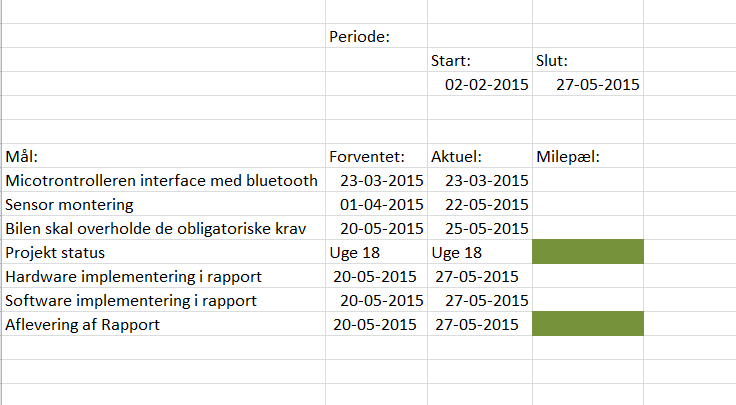
\includegraphics[scale=0.75]{Billeder/Tidsplan.PNG}
	\caption{Her kan vi se vores tidsplan}
	\label{fig:tidsplan}
\end{figure}